\chapter{Air Brakes, Resistance, and the v3 Simulator}
\label{ch:v3_sim}
\chaptermark{Air Brakes and the v3 Simulator}

% ---------------------------------------------------------------------------
% Part II, tier 2 of the plan in Ch. 10. Sources: SIMULATOR_VALIDATION_NOTE.md
% (log 2026-10-04 to 2026-10-16), simulator2/air_brake.py,
% simulator2/physics_config.py, simulator2/vehicle_physics.py,
% simulator2/power_assignment.py, simulator2/speed_planner.py.
% Numbers regenerate with:
%   python scripts/calibrate_air_brake.py          (fit, Wei out-of-sample)
%   python paper/scripts/plot_air_brake.py          (figure, rms per curve)
%   python scripts/air_brake_run_in.py              (Table tab:v3_run_in)
%   python scripts/build_dataset.py --physics v3 --n-scenarios 64 \
%       --batch-size 16 --seed 0 --out <dir>        (and --physics legacy;
%   python scripts/validate_dataset.py <dir>        Table tab:v3_smoke)
% ---------------------------------------------------------------------------

\Cref{ch:benchmark} gave the simulator a friction draft gear, notch traction and a dynamic brake, and showed that with the benchmark's inputs its in-train forces fall within the spread of six established simulators. That closed finding F3 of \cref{tab:critique_findings} and the form of F5. The benchmark could not test the rest. It excludes air brakes, so F1 and F2 were untouched; it supplies its own locomotives and resistance law, so the thesis's own consists still carried illustrative values; and it says nothing about F6 to F9, which concern standstill, grade, inertia and the scenarios themselves.

This chapter takes up those findings and assembles the result into one configuration, called v3, on which Part~III regenerates the corpus. Most of the chapter is the air brake, because it is the largest model added and because braking run-in, which the legacy corpora cannot contain, bears directly on the coupler-force constraint of the control problem. The remaining findings are smaller corrections, each tied to a source. The chapter ends with the problems that appeared only when everything was switched on together, and with what v3 does and does not establish.

\section{How a freight air brake works}
\label{sec:v3_brake_primer}

A freight train is braked by compressed air carried in a single pipe, the \emph{brake pipe}, that runs the length of the train through hoses between the cars. In the released state the locomotive keeps the pipe charged, at about 600\,kPa (90\,psi), and each car's reservoir is charged from it. The driver applies the brakes by \emph{reducing} the pipe pressure, venting air at the locomotive. Each car has a \emph{control valve} that senses the drop and admits air from the car's reservoir into its \emph{brake cylinder}, which presses the brake shoes against the wheels. The deeper the reduction, the higher the cylinder pressure, up to a \emph{full-service} application; a small reduction gives a \emph{minimum} application, about a third of full service \cite{Spiryagin2017HeavyHaul}. An \emph{emergency} application vents the pipe completely and is not modelled here.

Three features of this system matter for longitudinal dynamics.

\begin{itemize}
    \item \textbf{The brake is applied from the front.} The reduction starts at the locomotive and travels down the pipe, so the front cars brake first and the rear cars seconds later. Each control valve also vents a little pipe air locally when it first senses the reduction, a feature called \emph{quick service}, which speeds the reduction along the train. Even so, the pipe drains slowly over a long train, and the cylinders near the rear fill more slowly than those at the front.
    \item \textbf{The rear runs in against the front.} While the front is braked harder than the rear, the rear cars close up on the front ones and the couplers between them are compressed. This \emph{run-in} is the main source of compressive in-train force in braking.
    \item \textbf{The brake cannot be partly released.} North American control valves have \emph{direct release}: any increase in pipe pressure releases the car's brake completely \cite{Spiryagin2017HeavyHaul}. The brake cannot be applied again until the pipe and the reservoirs have recharged, which takes on the order of a minute or more.
\end{itemize}

Air brake models fall into two classes. Fluid-dynamic models solve the flow of air in the pipe and through each valve, and need the valve's internal geometry \cite{Specchia2012AirBrake}. Empirical models describe when and how fast each cylinder fills, and are calibrated to measured pressures. For studies in which the air brake is not itself the object, the review of \cite{Wu2016OverviewLTD} recommends the empirical class, and that is the class used here. The model has to reproduce the timing that causes run-in: when the brake reaches each car, and how fast its cylinder fills once it has.

\section{Brake timing}
\label{sec:v3_brake_timing}

\subsection{A first model, and why it failed}

The first model took the simplest form that has propagation at all. The brake command reaches a car at distance $d$ behind the locomotive after a delay $d/c$, and the car's brake force then rises with a first-order lag whose time constant grows linearly with $d$. Its timing was calibrated to the measured cylinder pressures of \cite{Wei2017AirBrake}, recorded on a 10,000\,t Chinese coal train of 116 cars. That gave a propagation speed of 176\,m/s, a time constant of 10.2\,s at the head of the train and 30.6\,s at the 116th car, an exhaust time constant of 6.7\,s on release, and a recharge time of 90\,s.

The model was then checked against a second source. \Cref{fig:v3_air_brake} shows its four panels: pipe and cylinder pressures recorded on a 100-wagon train with about 2,000\,m of brake pipe, at three positions along it, for minimum and full-service applications, with the pipe exhausted at the head only and at both ends \cite[Figs.~5.67--5.68]{Spiryagin2017HeavyHaul}. The curves were digitized from the book's vector graphics. At the head of the train the two sources agree: the cylinder time constant is 9.7\,s, against 10.2\,s from \cite{Wei2017AirBrake}. Behind the head they do not. The fitted time constant is 55\,s at 996\,m and 62\,s at 1,996\,m, where the linear model predicts 25 and 40\,s. The cylinders behind the head do not fill at a rate set by their own valves. They follow the pipe, which at 996\,m and 1,996\,m is still above 385\,kPa ninety seconds into a full-service application, against 350\,kPa at the head. The lag is front-loaded along the train and saturates with distance, which a time constant linear in distance cannot describe. The propagation speed differed too: the wave arrives at 266 to 273\,m/s on this train, inside the 250 to 300\,m/s the book gives for a well-designed system, against 176\,m/s on the Chinese train.

\subsection{The brake pipe model}

The model used instead describes the mechanism the second source points to: the cylinders are limited by the pipe. Let $u(t)$ be the driver's brake level, as a fraction of a full-service reduction, and let all pressures be carried as fractions of full service. For a car at pipe distance $d$ behind the locomotive:

\begin{enumerate}
    \item \textbf{The front.} The reduction reaches the car at $t_a = d/c$, with $c = 270$\,m/s. When it arrives, quick service vents a fixed share $q$ of a full-service reduction locally.
    \item \textbf{The pipe.} The rest of the reduction spreads along the pipe from the locomotive. The reduction $w(x,t)$ is modelled as linear diffusion,
    \begin{equation}
        \frac{\partial w}{\partial t} = D\,\frac{\partial^2 w}{\partial x^2},
        \qquad w(0, t) = u(t),
        \qquad \frac{\partial w}{\partial x}(L, t) = 0,
        \label{eq:v3_pipe}
    \end{equation}
    held at the driver's level at the locomotive and with no flow at the far end of a pipe of length $L$. (With the pipe also exhausted at the rear, the second condition becomes $w(L,t) = u(t)$.) The equation is linear, so its solution at each car is an exact sum of first-order lags with time constants $\tau_k = 4L^2/\bigl((2k-1)^2\pi^2 D\bigr)$. The slowest, $4L^2/(\pi^2 D)$, grows with the square of the pipe length.
    \item \textbf{The local reduction.} The car's pipe reduction is the larger of the quick-service share and the diffused reduction $w(d,t)$, and never more than the level that has arrived.
    \item \textbf{The control valve.} The cylinder fills towards the local reduction, quickly up to an \emph{inshot} level $\beta$ at rate $\rho_1$, and then at a slower, choke-limited service rate $\rho_2$. It only ever fills while the brake is applied: when the reduction is held, the valve laps and the cylinder holds its pressure.
    \item \textbf{Release.} A release travels down the pipe at its own speed, $c_r = 162.5$\,m/s. When it reaches a car the brake releases fully, and the cylinder exhausts with a time constant of 6.7\,s. The brake can be applied again 90\,s later, once the pipe has recharged.
\end{enumerate}

Distances are measured along the pipe, which is longer than the train because of the hoses and the piping on each car; the sources measure in pipe metres. Vehicle positions are converted with a pipe length factor of 1.081 metres of pipe per metre of train, the ratio for the consists of a published braking study \cite{NTSB2015Casselton}. The brake force on each car is its cylinder level times the car's full-service brake force, which is the subject of \cref{sec:v3_brake_force}.

\subsection{Calibration and checks}

The five pipe and valve parameters, $D$, $q$, $\beta$, $\rho_1$ and $\rho_2$, were fitted together to all eleven measured cylinder curves of the second source. \Cref{tab:v3_brake_timing} lists every timing parameter and where it comes from, and \cref{fig:v3_air_brake} shows the fit. The overall root-mean-square error is 15.9\,kPa on a full-service pressure of 350\,kPa, and 2.3 to 5.3\,kPa for the cylinders at the head. The fitted diffusivity puts the slowest pipe mode of a 2,000\,m pipe at 65\,s.

\begin{table}[htbp]
    \centering
    \small
    \begin{tabular}{>{\raggedright}p{5.0cm}r>{\raggedright\arraybackslash}p{6.2cm}}
        \toprule
        Parameter & Value & Source \\
        \midrule
        Front speed, $c$ & 270\,m/s & Onset waves, \cite[Fig.~5.67]{Spiryagin2017HeavyHaul} \\
        Pipe diffusivity, $D$ & 24,800\,m$^2$/s & Fitted, \cite[Figs.~5.67--5.68]{Spiryagin2017HeavyHaul} \\
        Quick-service share, $q$ & 0.187 & Fitted, same \\
        Inshot level, $\beta$ & 0.194 & Fitted, same \\
        Inshot rate, $\rho_1$ & 0.130 per s & Fitted, same \\
        Service rate, $\rho_2$ & 0.043 per s & Fitted, same \\
        Release speed, $c_r$ & 162.5\,m/s & Measured on a 150-wagon test rig \cite{Wu2017AirBrakeParallel} \\
        Exhaust time constant & 6.7\,s & \cite[Fig.~5]{Wei2017AirBrake} \\
        Recharge time & 90\,s & \cite{Wei2017AirBrake} \\
        Pipe length factor & 1.081 & \cite[Table~4]{NTSB2015Casselton} \\
        \bottomrule
    \end{tabular}
    \caption{Timing parameters of the air brake model. Levels and rates are fractions of a full-service application.}
    \label{tab:v3_brake_timing}
\end{table}

\begin{figure}[htbp]
    \centering
    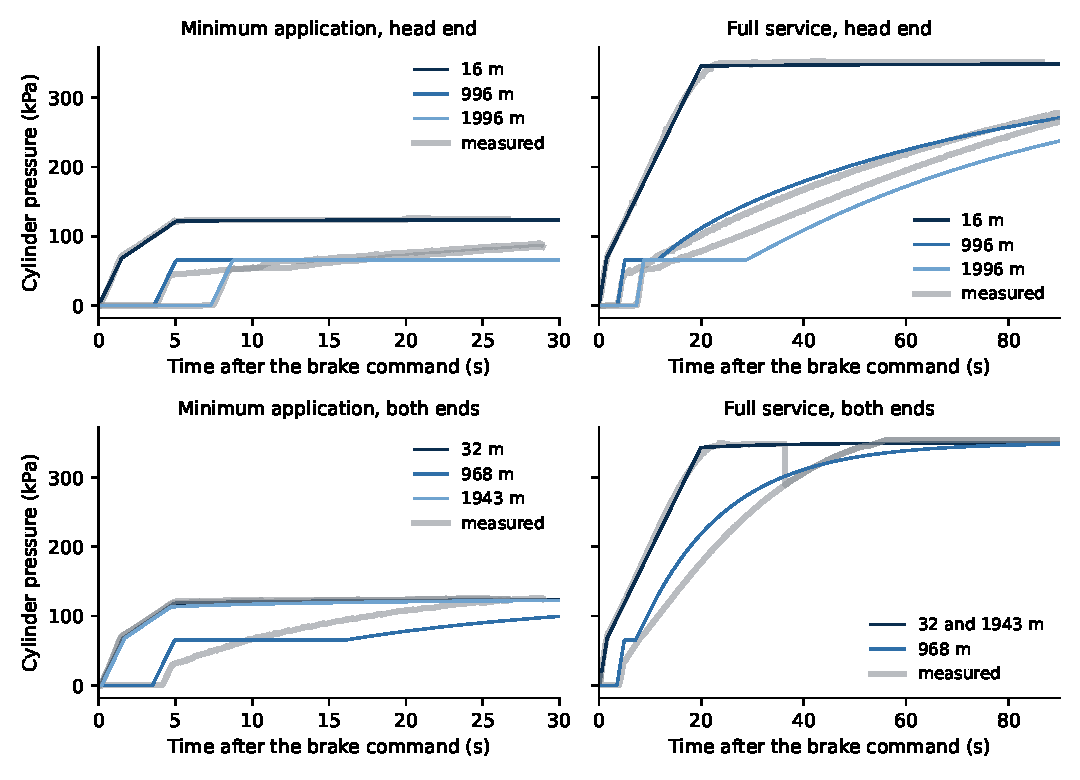
\includegraphics[width=\textwidth]{figures/air_brake_calibration.pdf}
    \caption{Brake cylinder pressure at three positions along a brake pipe of about 2,000\,m, measured \cite[Figs.~5.67--5.68]{Spiryagin2017HeavyHaul} (grey) and from the model with the parameters of \cref{tab:v3_brake_timing} (blue). Top: pipe exhausted at the head. Bottom: exhausted at both ends, so the two end cylinders coincide in the full-service panel.}
    \label{fig:v3_air_brake}
\end{figure}

The fit has one systematic residual. Behind the head, the model's cylinders end 20 to 28\,kPa low at the end of the minimum applications, and at 1,996\,m in full service. The measured rear cylinders fill faster than linear diffusion allows, which may be nonlinearity in the pipe flow or valve venting the model does not include.

Two independent checks support the fitted model. Without any refit, it predicts the measured cylinder of the 116th car of \cite{Wei2017AirBrake}, a different train, valve and pipe length, to 10.5\,kPa root-mean-square. One diffusivity therefore describes a 2\,km and a 1.4\,km pipe, which the linear first model could not. The 4th car of the same train is 26.7\,kPa off: near the head, where the pipe does not limit the cylinder, the fill is set by the valve itself, and the Chinese valve fills differently in detail from the one the fit follows. And the measurements of \cite{Wu2017AirBrakeParallel} put the quick-service dip in the pipe at 0.18 to 0.24 of a full-service reduction, around the fitted 0.187.

Twenty-five tests check the implementation. They compare the pipe solution with an independent finite-difference solve, with the pipe exhausted at the head and at both ends; check that the pipe lag scales with the square of its length; check the head cylinder against its closed form and the default parameters against one measured curve; and check that, integrated through the simulator, uncoupled cars lose exactly the impulse their commands imply and a coupled train's momentum follows the summed brake force to $10^{-7}$. Removing the pipe lag, the front delay or the valve's rate limit each makes at least one test fail.

\subsection{Limitations of the timing}

The fit rests on one train whose railway and valve the source does not name. The out-of-sample check is a Chinese train with the 120 valve, and the release speed comes from a Chinese test rig. None of the measurements is of the North American ABDX valve, so the model is a calibrated description of freight brake timing in general, not of a particular North American car. Propagation speed was a choice between sources, 176\,m/s and 270\,m/s; the second is used because it falls in the range the literature gives for a well-designed system and because the first depends on an unsourced car length. Emergency applications, which are faster and uniform along the train, are not modelled.

\section{Brake force}
\label{sec:v3_brake_force}

% ---------------------------------------------------------------------------
% PLACEHOLDER, held at the author's request (2026-10-16) until the
% outstanding requests are answered: AAR (S-401, brake design requirements;
% M-926, composition shoes) and a railroad (event-recorder data,
% paper/outreach/data_request_proposal.tex).
%
% For the eventual text. The model form is settled:
%   car shoe force = min(NBR x GRL, max empty ratio x actual weight);
%   retarding force = shoe friction x shoe force x g, capped at adhesion on
%   the vehicle's actual weight; locomotives use NBR on their own weight.
%   NBR is the actual normal shoe force over weight on rail, measured at the
%   shoe, so rigging losses are inside it (Snyder et al. 2000).
%   F1 reframed: a conventional car's shoe force is fixed by its rigging,
%   so load independence is right; the defects were the 250 kN magnitude
%   and the missing caps.
% Interim values in simulator2/air_brake.py (AirBrakeParams), from public
% documents quoting S-401:
%   NBR 0.10 (NTSB 2015 nominal fleet value; S-401: 11-14 % for cars built
%     after 2004, 8.5-13 % before);
%   GRL 286,000 lb = 129,727 kg (Snyder et al. 2000, Table 2);
%   max empty braking ratio 0.38 (S-401-99 via Snyder Table 1; NTSB fn. 4);
%   shoe friction 0.30 (Sun et al. 2024: AAR loaded form 0.32 - 0.002 V/3.6,
%     mean over 0-80 km/h);
%   adhesion 0.25, wet rail (Sun et al. 2024, Fig. 5);
%   pipe length factor 1.081 (NTSB 2015 Table 4; already cited above).
% Consequences: loaded 286k car 38.2 kN (0.29 m/s^2); 26 t empty 29.1 kN,
% set by the empty limit, not adhesion. Loaded adhesion demand <= 0.045,
% empty <= 0.12, so the adhesion cap binds only on bad rail. NBR is not
% randomized per car (8.5-14 %), which the NTSB study notes raises in-train
% forces when it varies.
% When the values are final, rerun scripts/air_brake_run_in.py and the
% smoke corpus of sec:v3_smoke; both use the interim capacity.
% ---------------------------------------------------------------------------

\emph{This section is held until outstanding requests for the brake design standard of the Association of American Railroads and for measured operating data are answered.} It will give the model of each car's full-service brake force, which converts the cylinder level of \cref{sec:v3_brake_timing} into a retarding force, and the parameter values it uses. The form of the model is settled; the values are not yet final. The results of \cref{sec:v3_run_in,sec:v3_smoke} use interim values and will be regenerated with the final ones.

\section{Braking run-in, measured}
\label{sec:v3_run_in}

\Cref{ch:critique} argued that the legacy corpora cannot contain braking run-in on uniform consists, because every car brakes at the same instant. With the brake pipe model that can now be measured directly. A uniform train of loaded 100\,t cars on a 15\,m pitch, running at 20\,m/s on level track, takes a full-service application. The run is repeated with the brake reaching every car at once, as in the legacy model, and with the brake pipe of \cref{sec:v3_brake_timing}, for two train lengths and both coupler models (\cref{tab:v3_run_in}).

\begin{table}[htbp]
    \centering
    \small
    \begin{tabular}{rlcc}
        \toprule
        Cars & Coupler & Every car at once & Brake pipe \\
        \midrule
        60  & Kelvin--Voigt (legacy) & 0 & 281 \\
        60  & Friction draft gear    & 0 & 178 \\
        130 & Kelvin--Voigt (legacy) & 0 & 828 \\
        130 & Friction draft gear    & 0 & 702 \\
        \bottomrule
    \end{tabular}
    \caption{Peak compressive coupler force (kN) in a full-service application from 20\,m/s, on uniform trains of 100\,t cars.}
    \label{tab:v3_run_in}
\end{table}

With every car braking at once the couplers carry no compressive force at all: every car decelerates at the same rate and nothing closes up. With the brake pipe, the same application produces several hundred kilonewtons. The force grows faster than the train's length, from 178 to 702\,kN on the draft gear as the train goes from 60 to 130 cars, because the pipe lag grows with the square of the pipe length and a longer train has more mass running in behind the front. The friction draft gear carries less than the legacy coupler, because it dissipates energy as the train closes up. This is the content the legacy corpora lacked and that a surrogate trained on them could not have learned.

\section{Resistance, locomotives and the smaller findings}
\label{sec:v3_findings}

\subsection{Running resistance (F4)}

The legacy model used fixed Davis coefficients per car type. v3 computes them for each vehicle from its mass and number of axles with the modified Davis equation for North American equipment \cite[Table~13.3]{Cole2019HandbookLTD},
\begin{equation}
    R = K_a\left(2.943 + \frac{89}{m_a} + 0.0305\,V + \frac{1.718\,k_{ad}\,V^2}{m_a\,n}\right)\ \text{N per tonne},
    \label{eq:v3_modified_davis}
\end{equation}
with $m_a$ the axle load in tonnes, $n$ the number of axles, $V$ the speed in km/h, $K_a$ an equipment factor (0.85 for most post-1950 cars, 1.05 for hoppers, 0.95 for container cars) and $k_{ad}$ an aerodynamic factor (0.07, or 0.0935 for containers). This is the law of the benchmark, \cref{eq:bench_resistance}, which the simulator was validated against in \cref{ch:benchmark}, including its factor of 3.2 on the leading locomotive.

The change is smaller than finding F4 suggested. F4 compared the legacy values with Davis's original formulae, which describe the plain-bearing equipment of the 1920s. Against the modified equation, which describes modern roller-bearing cars, the legacy values are close in the first two terms: for a loaded 120\,t hopper the modified equation gives $A = 745$\,N and $B = 13.8$\,N\,s/m, against the legacy 600\,N and 12\,N\,s/m. The real difference is in the aerodynamic term, $C = 1.64$\,N\,s$^2$/m$^2$ against 0.65, and in the lead locomotive, whose resistance the benchmark's factor more than triples.

\subsection{Locomotives and power (F5)}

\Cref{ch:benchmark} built notch traction and a dynamic brake but ran them on the benchmark's own locomotives. v3 gives the thesis's consists sourced ones (\cref{tab:v3_locos}). The illustrative SD70 becomes an SD70ACe and the illustrative GP38 an ES44DC, both six-axle road locomotives tabulated in \cite[Ch.~2]{Spiryagin2017HeavyHaul}. The GP38 is a four-axle unit. The book tabulates no four-axle unit, so the ES44DC, a six-axle road locomotive, stands in for it; the lighter locomotive of the legacy library is therefore considerably stronger under v3, and the power sizing of \cref{eq:v3_power_sizing} assigns fewer units in compensation.

\begin{table}[htbp]
    \centering
    \small
    \begin{tabular}{lcc}
        \toprule
        & SD70ACe & ES44DC \\
        \midrule
        Mass & 195\,t & 189.6\,t \\
        Starting tractive effort & 850\,kN & 632\,kN \\
        Continuous tractive effort & 698\,kN at 14.2\,km/h & 470\,kN at 21\,km/h \\
        Traction power & 3,207\,kW$^{a}$ & 3,274\,kW \\
        Dynamic brake, maximum & 472\,kN & 332\,kN \\
        Dynamic brake power & 5,500\,kW$^{a}$ & 3,875\,kW$^{b}$ \\
        \bottomrule
    \end{tabular}
    \caption{Sourced locomotives \cite[Tables~2.3 and 2.9]{Spiryagin2017HeavyHaul}. $^{a}$From the benchmark's type~2 locomotive, the same 195\,t, 850\,kN unit \cite{Spiryagin2017BenchmarkQuestions}, since the book gives no traction power. $^{b}$Derived: the maximum dynamic brake force at 42\,km/h, the speed where the tabulated curve leaves its plateau.}
    \label{tab:v3_locos}
\end{table}

Two consequences followed. The first is that the notch must not rise too fast. The regime library of \cref{sec:dataset_regimes} ramps traction freely, and with the stronger locomotives a ramp from notch 2 to notch 8 within seconds of a brake release ran a 142-car train out to 6.6\,MN. v3 lets the notch rise by at most one step every 8\,s, the fastest rate in the benchmark's driving \cite[Appendix~2]{Spiryagin2017BenchmarkQuestions}, and lets it fall at once. The dynamic-brake descent regime, which had driven the air brake as a stand-in, now uses the dynamic brake.

The second is that the trains now carry too much power. The consists were generated with locomotive counts sized for the illustrative 300\,kN and 180\,kN units, and the sourced units are two to three times stronger. v3 therefore re-sizes each scenario's power for the corridor it runs on, the way a railroad assigns power: the fewest units whose combined continuous tractive effort holds the whole train at their minimum continuous speed on the corridor's ruling grade,
\begin{equation}
    n\,T_{\mathrm{cont}} \ge \sum_i \Bigl( R_i(v_{\mathrm{cont}}) + m_i\,g\,\sin\theta_{\mathrm{rule}} \Bigr),
    \label{eq:v3_power_sizing}
\end{equation}
where the ruling grade $\theta_{\mathrm{rule}}$ is the steepest climb averaged over the train's length anywhere on the corridor. A train keeps its layout: a distributed-power train keeps at least one locomotive at the head and spreads the rest over its remote positions. Over 500 trains on five corridors the mean count falls from 2.53 to 1.66 locomotives. The rule is a minimum: it sizes a train that can just climb the ruling grade at 14 to 21\,km/h. On easy corridors that can be one locomotive for 13,000\,t, slower to accelerate than a railroad would accept for schedule. A floor in horsepower per trailing ton would correct that, but needs a source.

\subsection{Standstill (F6)}

The legacy resistance changes sign with speed and has no static friction, so a stopped car chatters about zero speed and nothing holds a stopped train on a grade; a braked car on a 1\% grade crept backwards at about 3\,cm/s. v3 adds static friction with the method of \cite{Karnopp1985StickSlip}. Below 0.1\,m/s a vehicle is held by a friction force that may be as large as its brake force plus a starting resistance of 34.3\,N per tonne, the lower of the values for roller bearings in \cite[p.~468]{Cole2019HandbookLTD}. Within that limit the friction cancels the driving force and brings the vehicle to rest within 0.1\,s; beyond it the vehicle breaks away and the friction stays at its limit. The first implementation left the holding force unbounded, so a held car anchored a train that should have crept; the bound is now pinned by a test.

\subsection{Grade and inertia (F7, F9)}

The grade force is now $mg\sin\theta$, removing the double sine of F7. Each vehicle's inertia is $m(1 + J_f)$, where $J_f$ is the rotating mass of wheelsets, gears and motors as a share of the vehicle's mass, 1.5\% for wagons and 12.5\% for locomotives, the midpoints of the ranges in \cite[p.~459]{Cole2019HandbookLTD}. Grade is still evaluated at each vehicle's centre rather than averaged over its length, which matters only where grade changes within a car length.

\section{Driving within the speed limit (F8)}
\label{sec:v3_planner}

The driving commands of the corpus are open loop: the regime library of \cref{sec:dataset_regimes} fixes each scenario's traction and brake commands in advance, without regard to the route, and the batch integrator needs them fixed in advance. In \texttt{data/v2}, 17.8\% of scenarios exceeded the speed limit by more than 5\,m/s as a result (\cref{sec:critique_data}).

v3 keeps the commands open loop but shapes them before the full simulation with a \emph{speed planner}. The planner simulates the train as a single mass along its route, with grade taken at every vehicle's position, under the regime's commands, and governs them:

\begin{itemize}
    \item \textbf{Allowed speed.} The limit that binds at a point is the lowest limit anywhere under the train, since the rear must clear a restriction too, backed off ahead of each lower limit by a braking curve at 0.15\,m/s$^2$, the low end of typical train decelerations \cite[p.~515]{Cole2019HandbookLTD}.
    \item \textbf{Governor.} Approaching the allowed speed, traction is reduced at a finite rate, as a driver notches off. Above it, the dynamic brake comes in, and beyond that a minimum air brake application is latched and released well below the limit, never sooner than the recharge time after the previous release.
    \item \textbf{Holding at a stop.} If the train is stopped or nearly so and the commanded traction cannot overcome grade and resistance, it is held on a full-service application. A minimum application was tried first, and let a 10,000\,t train on a 1.1\% grade roll back to 4.6\,m/s while the pipe filled.
    \item \textbf{No power against the brakes.} While the train is held, and after any release until the release has reached the rear and the cylinders have exhausted, traction is capped at notch 2. Powering up while the rear was still braked snatched a 143-car train to 7.6\,MN.
\end{itemize}

The regime's commands are replaced by the governed ones only where the governor acts, so each regime keeps its character away from the limits. The planner's model is cruder than the simulator's: it has no slack, no brake propagation and no notch lag, and margins in the governor absorb the difference.

One difference could not be absorbed, and it was found while this chapter was being written. The notch rate limit of \cref{sec:v3_findings} is applied after the planner, and the planner had been simulating the notches it commanded rather than the ones the train would get. In one smoke-test scenario, an 873\,t train on one locomotive under a 5.4\,m/s limit on grades up to 3.5\%, the governor cycled traction on and off to stay under the limit. The rate limit cut the delivered mean notch from 2.75 to 1.98, the train stalled on the grade, and because the planner's own train had not stalled, nothing held it. It rolled back 2\,km at up to 20\,m/s. The planner now applies the same rate limit to its own notches, through a step function shared with the command stage so that the two cannot drift apart, and a test checks that a command cycling between notch 0 and notch 8 accelerates the planner's train no faster than a steady notch 1. As a backstop, a v3 corpus build refuses any run in which a vehicle runs backwards faster than 1\,m/s, as it refuses runs whose couplers would have failed (\cref{sec:v3_assembly}).

\section{Assembling v3}
\label{sec:v3_assembly}

Every correction is selected by a single physics configuration, written into each scenario file and into the corpus manifest. The legacy configuration reproduces \texttt{data/v1} and \texttt{data/v2} exactly, so the Part~I data, its validator and the surrogate continue to work unchanged. \Cref{tab:v3_config} summarizes v3.

\begin{table}[htbp]
    \centering
    \small
    \begin{tabular}{>{\raggedright}p{0.7cm}>{\raggedright}p{4.6cm}>{\raggedright\arraybackslash}p{8.0cm}}
        \toprule
        & Legacy & v3 \\
        \midrule
        F1 & 250\,kN on every vehicle & Fixed shoe force per car, capped; values pending (\cref{sec:v3_brake_force}) \\
        F2 & Every car brakes at once & Brake pipe model, calibrated to measured cylinder pressures (\cref{sec:v3_brake_timing}) \\
        F3 & Kelvin--Voigt coupler & Friction draft gear on the benchmark's curve, 10\,mm slack (\cref{ch:benchmark}) \\
        F4 & Fixed Davis coefficients & Modified Davis per vehicle, lead factor 3.2 \\
        F5 & One force and power limit & SD70ACe and ES44DC, notches, dynamic brake, notch-up limit, power sized for the ruling grade \\
        F6 & No static friction & Static friction and starting resistance \\
        F7 & $mg\sin(\sin\theta)$ & $mg\sin\theta$ \\
        F8 & Speed limit ignored & Speed planner \\
        F9 & No rotating mass & Rotating mass; grade still at the vehicle centre \\
        \bottomrule
    \end{tabular}
    \caption{The legacy and v3 configurations against the findings of \cref{tab:critique_findings}.}
    \label{tab:v3_config}
\end{table}

Three problems appeared only when everything was switched on together.

\textbf{The integration step had to halve.} \Cref{sec:bench_step} found that the friction gear at its softer stiffness reproduces the benchmark at the legacy step of 0.02\,s. That held for the benchmark's loaded trains. When a gear reaches the end of its travel it meets a stiff end stop, $5\times10^{8}$\,N/m, and between two 26\,t empty cars that stop is a vibration of about 200\,rad/s. Fourth-order Runge--Kutta is stable only while the product of frequency and step stays below about 2.8, which at 0.02\,s allows 140\,rad/s. A 126-car v3 train diverged at 0.02\,s and ran cleanly at 0.01\,s, the step the benchmark comparison itself used, so v3 corpora are integrated at 0.01\,s. Runs that still go non-finite are not written.

\textbf{Trains had to start in equilibrium.} A scenario starts with its locomotives already at their first commanded notch. With the gears starting unloaded, four SD70ACe at notch 6 pulled about 20\,m of gear travel out of a 126-car train within seconds, and the rear snatched against the end stops at 8.8 to 14\,MN at every step size tried. A train running under that traction would already be stretched. v3 therefore starts each train in quasi-static equilibrium: it computes the force each coupler carries when the whole train accelerates as one, and sets each gear to the deflection and state that force requires. The peak force of that scenario fell to 2.4\,MN, and it no longer changes with the step size.

\textbf{Some trains would have parted.} The simulator has no coupler failure, so a run can carry forces a real knuckle would not survive. The rule was fixed before regeneration: a run whose peak coupler force exceeds the ultimate strength of a standard knuckle, 2.9\,MN \cite[p.~213]{Spiryagin2017HeavyHaul}, is not written, because that train would have parted. Runs between the knuckle's yield strength, 1.8\,MN, and its ultimate strength are kept and flagged. They occur in service, dropping them would bias the corpus towards gentle driving, and the control problem needs the surrogate to be accurate exactly where forces are high, so the surrogate's error on them is reported separately.

\subsection{A smoke test}
\label{sec:v3_smoke}

\Cref{tab:v3_smoke} compares a small corpus built with each configuration from the same random seed: the same 64 scenarios, the same consists, corridors and driving regimes. Both pass the corpus validator of \cref{sec:dataset_validation}.

\begin{table}[htbp]
    \centering
    \small
    \begin{tabular}{lcc}
        \toprule
        & Legacy & v3 \\
        \midrule
        Scenarios written & 64 & 64 \\
        Never over the speed limit & 73\% & 94\% \\
        Over the limit by more than 5\,m/s & 19\% & 0 \\
        Worst overspeed & 19.4\,m/s & 1.6\,m/s \\
        Running backwards faster than 1\,m/s & 28\% & 0 \\
        Fastest backward speed & 19.2\,m/s & 0.7\,m/s \\
        Highest coupler force & 1.40\,MN & 2.10\,MN \\
        Runs above knuckle yield (1.8\,MN) & 0 & 1 \\
        Mean locomotives per train & 2.45 & 1.72 \\
        Generation cost per scenario & 231\,ms & 978\,ms \\
        \bottomrule
    \end{tabular}
    \caption{The same 64 scenarios generated with the legacy and v3 configurations. Cost is per scenario in batches of 64 on one RTX~4090.}
    \label{tab:v3_smoke}
\end{table}

The v3 corpus keeps every train within 2\,m/s of the limit and none runs backwards faster than 0.7\,m/s; in the legacy corpus a fifth of the runs exceed the limit by more than 5\,m/s and over a quarter roll backwards faster than 1\,m/s. The highest coupler force is higher under v3. It comes from braking run-in, the force the legacy corpus could not produce: a 132-car train on a full brake application, which the regime library labels an emergency stop and the brake model applies as full service, reached 2.10\,MN, above the knuckle's yield strength, and is kept and flagged under the rule above. Each scenario costs about four times as much to generate: half of that is the shorter step, and the rest is the gear state and the notch law.

\section{What v3 establishes, and what it does not}
\label{sec:v3_scope}

Against the plan of \cref{sec:critique_plan}, v3 completes tier 2 except for the brake force values. Each correction has a source or a measured calibration, and the configuration as a whole contains the in-train force model that \cref{ch:benchmark} validated. What it has gained in fidelity it has paid for in cost and in the difficulty of the learning problem: the corpus now carries a gear state on every coupler, a different brake time constant on every vehicle, and notch tables on every locomotive.

The limits need stating as clearly as the gains.

\begin{itemize}
    \item \textbf{The brake force values are not final} (\cref{sec:v3_brake_force}).
    \item \textbf{The brake timing is not shown to be North American.} It is fitted to a train whose railway and valve are not named, and checked out of sample on a Chinese train with a Chinese valve. It describes freight brake timing well; it is not a model of the ABDX valve.
    \item \textbf{The configuration has not been validated as a whole.} The in-train force model was validated against other simulators with the benchmark's inputs, and the brake timing against measured pressures. No comparison exists of a v3 train against a real one. Requests for operating data from a railroad and for the brake standard were outstanding when this chapter was written; without them, tier 4 of the plan remains a stated limitation.
    \item \textbf{The driving is still synthetic.} The speed planner keeps open-loop regimes inside the limits; it is not a model of how drivers drive.
\end{itemize}

For the surrogate, v3 changes the learning problem in three ways. The coupler force now depends on each gear's history, so an edge must carry the gear state; each vehicle's brake responds with its own time constants; and each locomotive's force follows its notch table. \Cref{ch:surrogate_revised} takes up what that means for the model.

\section{Chapter summary}

The air brake was built twice. A first model, with a delay and a lag growing linearly along the train, was calibrated to one measured train and failed against a second: behind the head of the train the cylinders follow the brake pipe, not their own valves. The model used instead describes the pipe as linear diffusion behind a propagating front, with quick service and a two-rate control valve, and fits eleven measured cylinder curves to 15.9\,kPa root-mean-square on 350\,kPa, and predicts a cylinder of a second, Chinese train to 10.5\,kPa without refitting. With it, a full-service application on a uniform 130-car train produces 702\,kN of run-in on the friction draft gear, where the legacy model produces none. The brake force values are held pending outstanding requests.

The remaining findings were corrected from sources: modified Davis resistance, which turned out to differ from the legacy values mainly in the aerodynamic term; sourced SD70ACe and ES44DC locomotives, with a notch-up limit and power sized for each corridor's ruling grade; static friction; the exact grade force; and rotating mass. A speed planner shapes the open-loop commands to the speed limits, and a fault in it, which let a stalled train roll back unbraked, was found and fixed while this chapter was being written. Assembling the corrections required a step of 0.01\,s, an equilibrium start and a rule for trains that would have parted. The result, v3, is the configuration on which Part~III regenerates the corpus.
